\documentclass{mipt-thesis-ms}
% Следующие две строки нужны только для biblatex. Для inline-библиографии их следует убрать.
\usepackage{mipt-thesis-biblatex}
\addbibresource{main.bib}


\title{Исследование и разработка метода обратного инжиниринга истории построения трёхмерных моделей на основе структурной сегментации и машинного обучения}
\author{Егоров Г.\,А.}
\supervisor{TODO TODO.\,TODO.}
\referee{TODO TODO.\,TODO.}
\groupnum{М05-412д}
\faculty{Факультет прикладной математики и информатики}
\department{Кафедра технологий программирования игр}
\specialtynum{09.04.01}
\specialtytext{Информатика и вычислительная техника}


\begin{document}

\mainmatter
\pagestyle{miptthesis}
\titlepage \newpage
% META: TODO.1

\chapternoindex{Аннотация}

\textbf{Объём работы:} (TODO) страниц, включая (TODO) рисунков, (TODO) таблиц, (TODO) приложений. Библиографический список содержит (TODO) наименований.

\textbf{Ключевые слова:} машинное обучение, нейронные сети, CAD, КОМПАС-3D, обратный инжиниринг, история построения, сегментация 3D-моделей, MeshCNN, STEP, STL.

\textbf{Объект исследования:} процесс восстановления истории построения трёхмерных параметрических моделей в системе автоматизированного проектирования.

\textbf{Предмет исследования:} методы машинного обучения (глубокие нейронные сети для анализа трёхмерных сеток), применяемые для семантической сегментации геометрии и распознавания формообразующих операций, а также способы их интеграции с детерминированными алгоритмами CAD-ядра.

\textbf{Цель работы:} разработка программного модуля «НейроКОМПАС-3D», интегрируемого со средой КОМПАС-3D, который на основе анализа геометрии модели позволяет реконструировать последовательность породивших её операций.

\textbf{Методы исследования:} системный анализ, методы глубокого обучения (архитектура MeshCNN для классификации и сегментации), методы вычислительной геометрии (триангуляция, нормализация сеток, фильтрация), экспериментальное тестирование с количественным анализом метрик.

\textbf{Краткое содержание.} В работе проведён анализ предметной области, выявлены ограничения подхода прямого предсказания CAD-команд (высокая чувствительность регрессии параметров к шумам и системе координат). Обоснован и реализован гибридный подход, сочетающий нейросетевую сегментацию геометрии для распознавания следов операций (выдавливание, вырезание, скругление, фаска) с последующим детерминированным вычислением параметров средствами CAD-ядра.

Разработан конвейер подготовки датасета, позволяющий из сырых данных (истории построения в виде STEP файлов каждого шага + JSON-описание названий операций) автоматически генерировать размеченные по рёбрам OBJ-файлы. Исходный массив из (TODO)82 418 моделей после очистки и фильтрации сокращён до рабочего набора в (TODO)21 464 модели. На основе архитектуры MeshCNN обучены классификаторы и сегментаторы для четырёх основных операций: bossExtrusion, cutExtrusion, fillet, chamfer.

Экспериментально подтверждена состоятельность подхода согласно метрикам, измеренным на тестовой выборке после обучения. Точность классификации (accuracy, равное отношению числа верно классифицированных рёбер к общему числу рёбер) достигла: bossExtrusion - (TODO)\%, cutExtrusion - (TODO)\%, fillet - (TODO)90,6\%, chamfer - (TODO)\%. Метрика IoU: bossExtrusion - (TODO)\%, cutExtrusion - (TODO)\%, fillet - (TODO)\%, chamfer - (TODO)\%. Точность сегментации (accuracy): bossExtrusion - (TODO)\%, cutExtrusion - (TODO)\%, fillet - (TODO)\%, chamfer - (TODO)\%. Доля моделей, в которых минимум 90\% рёбер сегментированы верно, составила: bossExtrusion - (TODO)\%, cutExtrusion - (TODO)\%, fillet - (TODO)\%, chamfer - (TODO)\%.

Создан исполняемый модуль main.exe, реализующий полный цикл инференса: загрузку STEP / STL, адаптивную триангуляцию с бинарным поиском для ограничения числа треугольников (не более 1500), нормализацию сетки до фиксированного числа рёбер (2250), вызов нейросетевых моделей в автоматическом (перебор операций с исключением отвергнутых гипотез) или ручном режиме, постобработку (фильтрация треугольников по площади, выделение связного компонента) и подготовку выходных данных (STL-файл выделенной геометрии, JSON-файл с типом операции и уверенностью корректного её определения).

Модуль интегрируется с КОМПАС-3D через API, позволяя выполнять упрощение модели путём пошагового удаления распознанных операций. Разработанная архитектура допускает независимое дообучение классификаторов и сегментаторов, а также добавление новых типов операций без переучивания ранее добавленных, что даёт модульность и возможность улучшения результатов только для необходимых типов операций.

\textbf{Структура работы.} В первой главе проведён анализ предметной области, формализована задача, обоснован выбор гибридного подхода и нейросетевой архитектуры MeshCNN. Во второй главе описана архитектура решения: конвейер подготовки данных, схемы обучения и инференса, требования к форматам представления, а также приведены результаты экспериментального обучения и тестирования, а также сформулированы предложения по дальнейшему развитию (увеличение датасета, поддержка дополнительных операций, улучшение постобработки). (TODO)В приложениях вынесена техническая документация по установке, настройке и эксплуатации, а также примеры работы модуля на типовых деталях.

\textbf{Практическая значимость.} Разработанный модуль может быть использован для упрощения сложных 3D-моделей, восстановления параметрической истории импортированных моделей и обучения инженеров-конструкторов. Результаты работы внедрены в опытную эксплуатацию в рамках договора с ООО «АСКОН-Системы проектирования».

 \newpage
\tableofcontents \newpage
\chapternoindex{Введение}

Современное машиностроительное проектирование невозможно представить без использования систем автоматизированного проектирования (САПР), таких как КОМПАС-3D. Ключевым преимуществом параметрического моделирования является наличие истории построения — дерева операций, отражающего последовательность создания трёхмерной модели. Однако при работе с импортированными моделями (например, в формате STEP) или моделями, полученными от сторонних разработчиков, эта история часто отсутствует. Инженер получает лишь «немую» геометрию, что существенно затрудняет её редактирование, параметризацию и повторное использование. Задача восстановления истории построения по финальной геометрии, известная как обратный инжиниринг конструктивной истории, является крайне актуальной для промышленности. Она позволяет не только понять логику создания изделия, но и адаптировать его под новые требования, исправить ошибки или использовать в качестве основы для новых разработок.

Однако данная задача является нетривиальной даже с фундаментальной точки зрения. Одна и та же итоговая форма может быть получена различными последовательностями операций, а локальные изменения геометрии могут иметь множество параметрических интерпретаций. Традиционные алгоритмические методы часто оказываются неэффективны из-за высокой вариативности и сложности трёхмерных форм. В последние годы методы машинного обучения, особенно глубокие нейронные сети, показали впечатляющие результаты в анализе трёхмерных данных. Тем не менее, прямое применение существующих подходов для восстановления именно \textit{истории построения} наталкивается на ряд ограничений, связанных с необходимостью предсказывать не только тип операции, но и её точные числовые параметры.

\textbf{Целью} данной выпускной квалификационной работы является разработка программного модуля «НейроКОМПАС-3D», интегрируемого со средой КОМПАС-3D, который на основе анализа геометрии модели позволяет реконструировать последовательность породивших её операций с использованием методов машинного обучения.

Для достижения поставленной цели необходимо решить следующие \textbf{задачи}:
\begin{enumerate}
    \item Провести анализ предметной области, включая форматы представления трёхмерных данных (STEP, STL) и способы описания операций построения (Steps.txt, JSON), а также существующие подходы к анализу 3D-геометрии нейросетевыми методами.
    \item Сформировать требования к набору данных для обучения нейронной сети и подготовить (очистить, разместить) репрезентативный датасет, содержащий примеры моделей с известной историей построения.
    \item Исследовать различные архитектурные подходы к решению задачи, обосновать выбор наиболее перспективного гибридного подхода, сочетающего нейросетевую сегментацию и детерминированные алгоритмы CAD-ядра.
    \item Разработать и обучить нейросетевые модели (классификаторы и сегментаторы) для основных типов операций (выдавливание, вырезание, скругление, фаска) на базе архитектуры MeshCNN.
    \item Спроектировать и реализовать программный модуль, осуществляющий полный цикл инференса: загрузку модели, её предобработку, вызов нейросети, постобработку результатов и подготовку данных для интеграции с КОМПАС-3D.
    \item Провести экспериментальное тестирование разработанного модуля на реальных моделях, оценить точность распознавания и сегментации операций, выявить ограничения и предложить пути дальнейшего развития.
\end{enumerate}

\textbf{Объектом исследования} является процесс восстановления истории построения трёхмерных параметрических моделей. \textbf{Предмет исследования} — методы машинного обучения, применяемые для анализа геометрии и распознавания формообразующих операций в САПР.

В работе использовались следующие \textbf{методы исследования}: анализ научно-технической литературы и документации, системный подход к проектированию программных систем, методы машинного обучения (глубокие нейронные сети, в частности архитектура MeshCNN), методы обработки трёхмерной геометрии, экспериментальное тестирование и сравнительный анализ.

\textbf{Практическая значимость} работы заключается в создании действующего прототипа программного модуля, способного автоматизировать процесс реинжиниринга моделей в среде КОМПАС-3D. Модуль может быть использован для упрощения сложных моделей, восстановления параметров по импортированной геометрии и обучения работе с системой.

\textbf{Структура работы.} Выпускная квалификационная работа состоит из введения, трёх глав, заключения, библиографического списка и приложений. В первой главе проводится анализ предметной области, формализуется задача и обосновывается актуальность исследования. Вторая глава посвящена проектированию архитектуры решения, описанию структуры данных и выбору нейросетевых моделей. В третьей главе описывается программная реализация модуля, приводятся результаты экспериментального обучения и тестирования на реальных деталях, а также обсуждаются пути дальнейшего развития. В приложениях вынесена техническая документация и дополнительные иллюстративные материалы.


\chapternoindex{Основные понятия и сокращения}

В работе используются следующие термины и сокращения:

\begin{description}
    \item[API (Application Programming Interface)] – интерфейс программирования приложений.
    \item[B-Rep (Boundary Representation)] – метод представления трёхмерных тел в САПР.
    \item[\texttt{bossExtrusion}] – операция выдавливания (добавление материала).
    \item[CAD (Computer-Aided Design) / САПР] – система автоматизированного проектирования.
    \item[\texttt{chamfer}] – операция создания фаски.
    \item[\texttt{cutExtrusion}] – операция вырезания выдавливанием.
    \item[DGCNN (Dynamic Graph CNN)] – архитектура нейронной сети для облаков точек.
    \item[\texttt{fillet}] – операция скругления рёбер.
    \item[JSON (JavaScript Object Notation)] – текстовый формат обмена данными.
    \item[MeshCNN] – нейросетевая архитектура для полигональных сеток.
    \item[OBJ] – формат файла для представления трёхмерной геометрии.
    \item[PointNet] – архитектура для классификации и сегментации облаков точек.
    \item[STEP (Standard for the Exchange of Product model data)] – стандарт обмена данными между САПР.
    \item[STL (Stereolithography)] – формат для хранения триангулированных моделей.
    \item[Steps.txt] – промежуточный текстовый формат описания операций.
    \item[Гибридная архитектура] – сочетание нейросетевых методов и детерминированных алгоритмов CAD-ядра.
    \item[Детерминированный алгоритм] – алгоритм с однозначным результатом для одних и тех же входных данных.
    \item[История построения] – последовательность формообразующих операций и их параметров.
    \item[КОМПАС-3D] – система трёхмерного моделирования компании АСКОН.
    \item[Обратный инжиниринг] – процесс воссоздания модели по готовому образцу.
    \item[Сегментация 3D-модели] – разбиение поверхности на области, соответствующие операциям.
\end{description}



\chapter{Анализ предметной области и постановка задачи}

TODO2

\subsection{Введение в проблематику}

Современное машиностроительное производство невозможно представить без использования систем автоматизированного проектирования (САПР). Такие системы, как КОМПАС-3D, SolidWorks, CATIA, NX и другие, стали основным инструментом конструктора, позволяя создавать сложные трёхмерные модели деталей и сборочных единиц с высокой точностью и производительностью. Ключевым преимуществом современных САПР является параметрическое моделирование — подход, при котором геометрия модели описывается не фиксированным набором точек и поверхностей, а последовательностью операций с изменяемыми числовыми параметрами и геометрическими ограничениями.

Однако на практике инженеры регулярно сталкиваются с ситуацией, когда параметрическая история построения модели недоступна. Это происходит при импорте моделей из нейтральных форматов (например, STEP или IGES), при получении моделей от сторонних организаций, использующих другое программное обеспечение, при работе с унаследованными базами моделей, созданных без соблюдения параметрической дисциплины, а также при получении геометрии с 3D-сканеров реальных физических объектов \cite{kim2023reconstruction}. В таких случаях инженер получает «немую» геометрию — статичное представление, из которого невозможно понять логику создания модели, невозможно изменить отдельные элементы, не перестраивая модель заново. Редактирование такой модели становится крайне трудоёмким, а часто и вовсе невозможным без полного перепроектирования.

Задача восстановления истории построения по финальной геометрии, известная как обратный инжиниринг конструктивной истории (Inverse CAD), является одной из наиболее сложных и востребованных задач в области промышленного программного обеспечения. Её решение позволило бы не только понимать логику создания изделия, но и эффективно адаптировать его под новые требования, исправлять ошибки, использовать существующие разработки в качестве основы для новых проектов, а также обучать начинающих специалистов на примерах реальных моделей \cite{autodesk2020}.

Традиционные алгоритмические методы анализа геометрии, основанные на поиске примитивов и распознавании поверхностей, имеют существенные ограничения. Одна и та же итоговая форма может быть получена различными последовательностями операций, а одно и то же локальное изменение геометрии может иметь множество параметрических интерпретаций \cite{isicad2013direct}. Более того, такие методы, как правило, производят искусственный, не свойственный человеку порядок операций, что затрудняет их практическое использование.

В последние годы методы машинного обучения, особенно глубокие нейронные сети, показали впечатляющие результаты в анализе трёхмерных данных (классификация, сегментация, генерация). Однако прямое применение существующих подходов для восстановления именно истории построения наталкивается на ряд фундаментальных ограничений, связанных с необходимостью предсказывать не только тип операции, но и её точные числовые параметры, чувствительные к масштабу, системе координат и дискретизации.

Данная глава посвящена систематическому анализу теоретических и технологических основ, необходимых для решения задачи восстановления истории построения CAD-моделей с использованием методов машинного обучения. В ней будут рассмотрены: принципы параметрического моделирования и структура истории построения, форматы представления трёхмерных данных (STEP и STL), современное состояние методов обратного инжиниринга в промышленности, а также обзор архитектур нейронных сетей для анализа трёхмерной геометрии — от облаков точек до сеточных представлений.



\section{Анализ существующих подходов и форматов данных}

TODO2

TODO3

Качество решения в задачах машинного обучения на инженерной геометрии почти полностью определяется качеством и организацией набора данных. В проекте «НейроКОМПАС-3D» датасет имеет структуру последовательностей: каждой модели соответствует папка, содержащая шаги построения. Для каждого шага доступны файлы STEP и STL, а также файл текстового описания операций между шагами; в более поздней редакции пайплайна используются JSON-метаданные. Такой формат воспроизводит реальную логику CAD-построения, где объект существует как история преобразований, а не как статичная сетка.

Требования к формату данных были зафиксированы уже на первом этапе. Для каждой модели должны быть доступны идентификатор набора, номера шагов, файл с описанием операций и согласованный словарь поддерживаемых операций. В финальной реализации в типовой набор операций вошли: выдавливание (bossExtrusion), вырезание выдавливанием (cutExtrusion), скругление (fillet), фаска (chamfer). Эта ограниченная номенклатура была выбрана осознанно: она позволяла локализовать исследование на наиболее типичных и одновременно существенно различающихся по геометрическим признакам операциях, не пытаясь сразу охватить весь спектр CAD-команд.

Важным элементом начальной постановки было понимание масштабов данных. Уже в ранних отчетных материалах указывалась ориентировочная потребность порядка 10 000 моделей по 20–30 шагов для этапов 2 и 3. Практика полностью подтвердила эту оценку. Первичная тестовая выборка из 362 наборов оказалась достаточной для демонстрации обучаемости, но недостаточной для достоверного сравнения архитектур и устойчивых выводов по качеству. Следовательно, в проекте изначально корректно оценивалась высокая data hunger задачи.

Особое внимание в проекте уделялось препроцессингу и численной нормализации. На этапе 3 STL-файлы преобразовывались в point cloud размерности N×3, геометрия переносилась в окрестность начала координат и масштабировалась к единичному размеру. Steps.txt разбирался на пары «ключ-значение»; ключи кодировались one-hot-векторами; значения нормировались в зависимости от типа — углы переводились в 0–1, длины домножались на коэффициент масштаба, координаты сдвигались на дельту переноса.

Отдельной проблемой стала координатная система операции и ее связь с глобальной системой модели. В рабочих материалах прямо отмечалась необходимость хранить нормаль к плоскости эскиза либо матрицу поворота и смещение, позволяющие сопоставить систему STL и систему эскиза. Это замечание отражает важную теорему инженерного машинного обучения: если модель должна предсказывать параметры в локальной системе объекта, то либо вход должен быть инвариантен к глобальному положению, либо ему необходимо явно сообщить преобразование между системами координат. Игнорирование этого принципа ведет к резкому падению качества регрессии.

Применительно к сегментационному варианту датасет претерпел существенную переработку. STEP стал использоваться не столько как прямой вход для сети, сколько как источник точной геометрической семантики при формировании меток. Для пары соседних шагов определялись изменившиеся грани; далее для треугольников финальной модели вычислялось соответствие типу операции, породившей содержащую их грань. Тем самым была реализована масштабируемая схема автоматической разметки без ручного аннотирования каждого треугольника человеком.

Вторая нейронная линия относится к сегментации. В качестве базового варианта была рассмотрена MeshCNN-модель, работающая по ребрам и локальным отношениям смежности. Для сложных поверхностей такая архитектура привлекательна тем, что использует топологию сетки, а не только набор несвязанных точек. В перспективе также рассматривались PointCNN и иные модели, способные обобщать представление до point cloud и лучше переноситься на геометрию с большим числом треугольников. Фактически в проекте был исследован спектр между сеточно-зависимыми и сеточно-инвариантными представлениями.



\section{Исследование существующих аналогов}

Задача восстановления истории построения трёхмерных моделей по их конечной геометрии (обратный инжиниринг конструктивной истории) является одной из ключевых проблем в области систем автоматизированного проектирования (САПР). Несмотря на то, что коммерческие CAD-системы традиционно используют параметрическое представление с историей построения, при обмене данными между различными платформами или при работе с унаследованными моделями эта информация часто теряется. Как отмечается в современной литературе, распространённые форматы обмена, такие как IGES, не поддерживают хранение истории построения, а даже стандарт STEP, хотя и предусматривает такую возможность, полностью не реализован в большинстве коммерческих систем \cite{kim2023reconstruction}. В результате инженеры получают так называемые «немые» (dumb) модели, представленные только в виде B-Rep (Boundary Representation) или триангулированной геометрии, что существенно затрудняет их редактирование, параметризацию и повторное использование.

Актуальность данной проблемы подтверждается как промышленными потребностями, так и активными исследованиями в этой области. По данным обзора Steininger и соавторов \cite{steininger2025enhancing}, применение методов генеративного искусственного интеллекта в САПР выделяется в четыре основных направления: генерация новых дизайнов, реконструкция существующих, поиск аналогов и модификация. Восстановление истории построения относится к области реконструкции, которая в последние годы демонстрирует наиболее интенсивное развитие благодаря успехам глубокого обучения.

\subsection{Промышленные решения для обратного инжиниринга}

На сегодняшний день наиболее распространённым коммерческим решением для восстановления параметрических признаков из импортированной геометрии является модуль FeatureWorks, входящий в состав САПР SOLIDWORKS \cite{solidxperts2025featureworks}. Данный инструмент позволяет распознавать типовые конструктивные элементы (отверстия, выдавливания, скругления, фаски) в импортированных STEP-, IGES- и Parasolid-файлах, после чего пользователь получает частично восстановленное дерево построения с возможностью редактирования параметров. FeatureWorks поддерживает как автоматический режим распознавания, так и интерактивный, где пользователь вручную указывает элементы для распознавания.

Однако, согласно анализу, представленному на официальном блоге SOLIDWORKS, данный инструмент имеет существенные ограничения \cite{solidxperts2025featureworks}. Во-первых, качество распознавания сильно зависит от сложности геометрии: для литейных форм, поверхностей сложной формы и органических объектов точность резко снижается. Во-вторых, FeatureWorks не восстанавливает эскизные ограничения и связи между параметрами, что ограничивает возможности дальнейшей параметризации. В-третьих, модуль не поддерживает работу со сборочными единицами — каждый компонент необходимо обрабатывать отдельно. Эти ограничения демонстрируют, что даже ведущее промышленное решение не обеспечивает полноценного автоматического восстановления истории построения, особенно для сложных моделей.

Следует отметить, что в экосистеме КОМПАС-3D, которая является целевой средой для разрабатываемого модуля «НейроКОМПАС-3D», на данный момент отсутствует встроенный инструмент, аналогичный FeatureWorks. Это создаёт дополнительную потребность в разработке собственного решения, учитывающего специфику форматов и операционной логики КОМПАС-3D.

\subsection{Академические исследования и перспективные подходы}

Академическое сообщество активно исследует проблему восстановления истории построения с использованием методов машинного обучения, и за последние годы был достигнут значительный прогресс. Обзор современных исследований позволяет выделить несколько ключевых направлений.

\subsubsection{Методы на основе традиционных алгоритмов}

Исторически первыми подходами к решению задачи были алгоритмические методы, основанные на декомпозиции геометрии. Среди них можно выделить методы максимальной декомпозиции объёмов (maximal volume decomposition), предложенные Сакураи \cite{sakurai1998maximal}, а также методы альтернативной суммы объёмов (alternating sum of volumes, ASV) и её модификации ASVP, разработанные Кимом и соавторами \cite{kim2000asvp}. Эти подходы позволяют преобразовывать B-Rep модель в представление в виде конструктивной сплошной геометрии (CSG), где форма описывается как последовательность булевых операций над простыми примитивами.

Однако, как отмечается в недавнем обзоре \cite{kim2023reconstruction}, алгоритмические методы имеют фундаментальные ограничения. Во-первых, они требуют значительных вычислительных ресурсов при работе со сложными моделями и могут не завершиться за приемлемое время. Во-вторых, они не способны распознавать параметры примитивов с высокой точностью. В-третьих, такие методы плохо масштабируются на широкий класс операций и не учитывают семантику конструктивных элементов.

\subsubsection{Методы глубокого обучения для распознавания признаков}

С развитием глубокого обучения исследователи обратились к нейросетевым подходам. Первые попытки использовали свёрточные нейронные сети для анализа воксельных представлений и облаков точек. Однако, как показано в работе Cao и соавторов \cite{cao2020brepnet}, такие аппроксимации неизбежно теряют точность геометрического описания и не позволяют в полной мере использовать топологическую информацию, содержащуюся в B-Rep представлении.

Прорывным направлением стало использование графовых нейронных сетей (GNN) для работы с графами смежности граней, непосредственно извлекаемыми из B-Rep моделей. Работа UV-Net \cite{jayaraman2021uvnet} предложила метод, в котором поверхности граней проецируются в UV-пространство для формирования двумерных сеток, обрабатываемых свёрточными сетями, после чего графовая нейронная сеть учитывает связи между соседними гранями. Аналогичный подход реализован в Hierarchical CADNet \cite{zhang2022hierarchical}, где используется иерархическое представление геометрии.

Люксембургская исследовательская группа под руководством Элоны Дюпон \cite{dupont2025design} представила систематическое исследование подходов к восстановлению истории построения. В своей диссертационной работе, защищённой в 2025 году, автор рассматривает несколько последовательных направлений: от восстановления элементов конструктивной истории из существующих B-Rep представлений до использования иерархических архитектур Transformer для прямого предсказания последовательности операций по облаку точек. Особый интерес представляет предложенный автором подход к использованию больших языковых моделей для генерации исполняемого Python-кода, описывающего процесс построения модели, что позволяет обойти ограничения, связанные с отсутствием стандартизированных форматов представления.

\subsubsection{Генерация параметрических моделей из изображений}

Отдельное направление исследований связано с генерацией CAD-моделей непосредственно из изображений. Работа CADCrafter \cite{chen2025cadcrafter}, представленная на конференции CVPR 2025, демонстрирует возможность создания полных CAD-файлов (в формате STEP) по единственному изображению объекта. Авторы используют комбинацию вариационных автоэнкодеров (VAE) и диффузионных моделей на основе архитектуры Transformer для генерации последовательностей CAD-инструкций. Особенностью подхода является введение механизма проверки компилируемости генерируемого кода с использованием DPO (Direct Preference Optimization), что позволяет существенно повысить долю успешно компилируемых и геометрически корректных моделей.

Это исследование демонстрирует принципиальную возможность использования современных архитектур глубокого обучения для решения задачи, сходной с обратным инжинирингом, хотя и в условиях, когда входные данные представлены в более структурированной форме (изображения), а не в виде трёхмерной геометрии.

\subsection{Проблема датасетов для обучения}

Ключевым препятствием для развития методов машинного обучения в области восстановления истории построения является отсутствие достаточных размеченных наборов данных. Как отмечается в обзоре \cite{steininger2025enhancing}, большинство существующих датасетов либо слишком малы, либо не содержат полной информации о последовательности операций построения.

Важным шагом в этом направлении стал выпуск Autodesk Fusion 360 Gallery Dataset \cite{autodesk2020fusion}, содержащего более 8 тысяч моделей с полной историей построения. Этот датасет, впервые представленный в 2020 году, стал основой для многих последующих исследований, включая работы \cite{dupont2025design} и \cite{chen2025cadcrafter}. Однако, как указывается в корейском исследовании по автоматической генерации датасетов \cite{kim2024automatic}, существующих данных всё ещё недостаточно для обучения моделей, способных обобщаться на широкий класс реальных инженерных задач. Авторы предлагают методы автоматической генерации синтетических датасетов на основе случайного комбинирования параметров признаков с наложением ограничений на реалистичность форм.

В рамках настоящей работы также была проделана значительная работа по формированию датасета: из исходного массива в 82 418 моделей после многоступенчатой фильтрации получен рабочий набор из 21 464 моделей, каждая из которых содержит STEP- и STL-представления, а также JSON-файл с подробным описанием всех операций построения. Это позволяет проводить обучение в supervised режиме и может рассматриваться как вклад в развитие открытых данных для данной предметной области.

\subsection{Анализ проблемы и обоснование необходимости разработки}

Проведённый анализ существующих решений и исследований позволяет выделить несколько ключевых выводов:

\begin{enumerate}
    \item \textbf{Отсутствие универсального промышленного решения.} Даже ведущие CAD-системы, такие как SOLIDWORKS с модулем FeatureWorks, предлагают лишь ограниченные возможности по восстановлению истории построения, работающие преимущественно на простых геометриях и не восстанавливающие полную параметрическую связанность модели.
    
    \item \textbf{Необходимость адаптации под конкретную CAD-систему.} Каждая CAD-платформа имеет собственную систему типов операций, параметров и API, что делает невозможным прямое перенесение решений между системами. Для экосистемы КОМПАС-3D специализированное решение отсутствует.
    
    \item \textbf{Перспективность гибридных подходов.} Современные академические исследования \cite{dupont2025design} \cite{chen2025cadcrafter} демонстрируют, что наиболее эффективными являются гибридные архитектуры, сочетающие нейросетевые методы для распознавания геометрических паттернов и детерминированные алгоритмы для точной параметризации. Этот вывод согласуется с архитектурным решением, принятым в настоящем проекте.
    
    \item \textbf{Ключевая роль датасетов.} Успех применения методов машинного обучения напрямую зависит от наличия качественных размеченных данных. Существующие датасеты либо ограничены по объёму, либо не полностью соответствуют специфике конкретной CAD-системы.
    
    \item \textbf{Проблема точности параметров.} Как показано в исследовании Autodesk \cite{autodesk2020fusion}, нейросетевые методы хорошо справляются с определением типа операции и грубой локализацией, но точное восстановление численных параметров остаётся сложной задачей. Это подтверждает правильность выбранного в проекте подхода, при котором нейросеть отвечает за сегментацию, а точное вычисление параметров переносится на сторону CAD-ядра.
\end{enumerate}

На основе проведённого анализа можно заключить, что разработка программного модуля «НейроКОМПАС-3D» является актуальной и востребованной задачей. Предлагаемое решение, основанное на гибридной архитектуре с использованием нейросетевой сегментации геометрии и детерминированной постобработки средствами КОМПАС-3D, позволяет учесть специфику целевой CAD-системы и преодолеть ограничения существующих подходов.

\section{Формализация задачи как процесса обратного вывода конструктивной истории}

TODO2

В научно-техническом отношении задача проекта может быть формализована как задача обратного вывода конструктивной истории параметрической трехмерной модели. Пусть имеется последовательность состояний M0, M1, …, Mn, где каждый переход Mi→Mi+1 реализован некоторой операцией oi. Каждая операция обладает типом из словаря допустимых CAD-операций, параметрами, привязкой к геометрическим сущностям и местом в частично упорядоченной истории. Требуется по наблюдаемым данным Mk (где k >= i+1) восстановить отдельную операцию oi.

TODO3

Даже в таком компактном описании видно, что задача имеет гибридную природу. Пространство входов включает как дискретизированные поверхности STL, так и более точные топологические и параметрические описания STEP, а также текстовые или JSON-метаданные. Пространство выходов также неоднородно: тип операции является дискретной переменной; параметры включают непрерывные, целочисленные, булевы и категориальные величины; сегментация задает распределение меток по треугольникам, ребрам, граням или точкам; восстановление дерева построения требует последовательностной логики. Следовательно, простая редукция задачи к одной классификации или одной регрессии принципиально недостаточна.

Реализация проекта была построена в логике последовательности итерационных исследовательских циклов. Были рассмотрены два параллельных подхода: прямое предсказание операций и параметров по STL / текстового описания операций в формате Steps.txt, и альтернативный путь через классификацию и сегментирование каждой операции отдельно на основании STEP / текстового описания операций в формате JSON.



\section{Актуальность, цель и задачи исследования}

TODO2

Предметом работы является разработка программного модуля «НейроКОМПАС-3D», включающего обучаемые модели, средства подготовки данных, исполнительные сценарии инференса и интеграционный контур взаимодействия с КОМПАС-3D. В задаче присутствуют три взаимосвязанные подсистемы: дата-инженерный контур; нейросетевой контур; контур интеграции с CAD-средой.

Целью является разработка программного модуля «НейроКОМПАС-3D», включающего обучаемые модели, средства подготовки данных, исполнительные сценарии инференса и интеграционный контур взаимодействия с КОМПАС-3D. В задаче присутствуют три взаимосвязанные подсистемы: дата-инженерный контур; нейросетевой контур; контур интеграции с CAD-средой.

Задачи:

Определены поддерживаемые операции, формат набора данных, предложены CNN/Transformer/GNN-подходы. Разработаны требования к набору данных для машинного обучения. Сформированы первичные наборы данных для обучения нейронной сети. Разработана архитектура нейронной сети, пригодная для решения поставленных задач.

Разработан dataloader, выполнен препроцессинг, обучена базовая модель, подтверждена концептуальная возможность. Проведено предварительное обучение на основании подготовленного набора данных. Сформирован отчет с техническими показателями обучения нейронной сети и предложениями по дальнейшему улучшению показателей, в том числе с помощью корректировки архитектуры модели и исходных данных.

Подготовлены модели для Steps.txt и геометрии, оформлен комплект ПО и весов. Разработаны нейронные сети, которые способны формировать один шаг построения на основе двух моделей в определённом на этапе 1 формате (начальной и конечной), отличающихся одним элементарным построением  из набора элементарных операций, определённом на этапе 1.

Обоснован и принят сегментационный подход, обработан подготовленный специалистами Заказчика новый модифицированный крупный датасет, доработаны и обучены нейросети классификаторов и сегментаторов для каждого типа выбранных операций, разработан модуль main.exe (интегрируемый с КОМПАС-3D). Разработаны нейронные сети, которые способны пошагово (в итерационном взаимодействии с КОМПАС-3D) формировать промежуточные ветви дерева построения на основе двух моделей в определённом на этапе 1 формате (начальной и конечной), отличающихся несколькими элементарными построениями из набора элементарных операций, определённом на этапе 1.


\chapter{Проектирование архитектуры и методов решения}

TODO2

\section{Эволюция архитектурного подхода}

На раннем этапе исследования естественным вариантом было обучение системы напрямую предсказывать текстовую команду (Steps.txt) по двум состояниям модели – до и после элементарной операции. Однако эксперименты показали, что тип операции определяется достаточно надёжно, а точные численные параметры – значительно хуже. Это связано с чувствительностью параметров к масштабу модели, системе координат и дискретизации поверхности.

В качестве промежуточного решения была предложена модульная архитектура, где после извлечения признаков из двух STL выполнялась классификация типа операции, а затем специализированный блок регрессии предсказывал параметры. Однако точные числа по-прежнему трудно восстановить из дискретизированной геометрии.

Следующий шаг заключался в переосмыслении роли нейросети: вместо предсказания команд, она должна отвечать за распознавание геометрических паттернов и локализацию следов операций. Параметрическая реконструкция переносится на сторону CAD-ядра, где доступны точные геометрические вычисления. Такой подход, получивший название \textit{гибридная сегментационно-классификационная схема}, позволяет:
\begin{itemize}
    \item избежать прямой регрессии численных параметров;
    \item получить интерпретируемый результат в виде «раскраски» модели;
    \item итеративно применять и проверять гипотезы на стороне CAD;
    \item использовать специализированные сети для разных операций.
\end{itemize}

В таблице~\ref{tab:approach-comparison} приведено сравнение рассмотренных подходов.

\begin{table}[h]
\centering
\caption{Сравнение подходов к реализации}
\label{tab:approach-comparison}
\begin{tabular}{|p{4cm}|p{4cm}|p{4cm}|p{3.5cm}|}
\hline
\textbf{Подход} & \textbf{Преимущества} & \textbf{Ограничения} & \textbf{Итоговая оценка} \\
\hline
Прямое предсказание Steps.txt & Явный формат выхода; логичная интеграция через API & Высокая чувствительность к численным параметрам, системе координат и накоплению ошибки & Хорошая исследовательская гипотеза, но недостаточно устойчива \\
\hline
Модульная классификация + регрессия & Разделение типа операции и параметров; расширяемость по операциям & Параметры остаются труднорегрессируемыми из дискретизированной геометрии & Ценный промежуточный шаг \\
\hline
Сегментация полной геометрии & Соответствует природе 3D-данных; даёт интерпретируемый результат; позволяет перенести точные вычисления в CAD & Требует автоматической разметки и балансировки датасета по операциям & Наиболее перспективный подход на текущем этапе \\
\hline
Специализированные сети по операциям & Упрощение задачи; независимое дообучение; повышение управляемости качества & Нужна оркестрация результатов и отдельные выборки под каждый класс & Рекомендуемое направление развития \\
\hline
\end{tabular}
\end{table}



\section{Структура данных и требования к датасету}

TODO2

\subsection{Форматы входных данных и их препроцессинг}

В проекте ранее уже были практически проверены несколько представлений данных, такие как облака точек XYZ, возникающие при семплировании поверхности или объема, и промежуточный текстовый язык Steps.txt или .json, используемый для описания операций между соседними шагами построения. Но в текущем рабочем подходе используются несколько представлений, дополняющих друг друга. Первое — треугольные сетки STL, на которых можно строить CNN-подобные, графовые или меш-ориентированные модели. Второе — STEP/B-Rep-представление, потенциально пригодное для более глубокого анализа поверхностей, граней, топологии сопряжения и инженерной семантики, и необходимое для автоматической разметки датасета. Третье — промежуточный текстовый структурированный язык в формате JSON, используемый для описания операций между соседними шагами построения.

Таким образом, текущий рабочий подход предполагает использование нескольких представлений в зависимости от стадии конвейера. Для точного восстановления параметров и привязки к инженерному смыслу предпочтительнее STEP/B-Rep. Для разметки датасета и определения пригодности модели для обучения данной операции сохраняется промежуточное командное описание в виде JSON. Для первичного распознавания допустимы STL и производные от него представления.



\subsection{Формирование и очистка обучающей выборки}

Статистика подготовки нового массива данных показывает масштаб инженерной фильтрации. Из 82 418 исходно подготовленных моделей только 44 181 прошли первичную обработку. Далее были выявлены 18 моделей с двумя JSON-файлами, 262 без JSON, 7 417 без STL/STEP и 15 020 с единственной парой STL+STEP, непригодной для обучения переходов между шагами. В итоге рабочий набор составил 21 464 моделей. Эта статистика показывает, что управление качеством данных в проекте является не вспомогательной, а центральной функцией.

На частном эксперименте по операции fillet из всего итогового набора были отобраны только 1 726 моделей, одновременно содержащих скругление и не превышающих порог сложности в 1 500 треугольников. Данный факт важен по двум причинам. Во-первых, большой суммарный датасет не гарантирует достаточный объем примеров для каждой операции. Во-вторых, ограничения по сложности геометрии дополнительно уменьшают фактическую выборку и могут приводить к смещению модели в сторону упрощенных случаев. Следовательно, стратегией развития должен быть не просто рост общего количества моделей, а целевой набор сбалансированных подмассивов по операциям и уровням сложности.

\newpage
\begin{table}[h]
\centering
\caption{Статистика подготовки данных}
\label{tab:data-preparation-stats}
\begin{tabular}{|l|r|p{6cm}|}
\hline
\textbf{Показатель} & \textbf{Значение} & \textbf{Смысл для проекта} \\
\hline
Подготовлено моделей & 82 418 & Сырой массив, отражающий потенциал масштабирования \\
\hline
Прошли первичную обработку & 44 181 & Модели, достигшие стадии первичной машинной обработки \\
\hline
Два JSON & 18 & Структурная неоднозначность метаданных \\
\hline
Нет JSON & 262 & Невозможность supervised-разметки по операциям \\
\hline
Нет STL/STEP & 7 417 & Потеря геометрической основы для обучения \\
\hline
Только одна пара STL+STEP & 15 020 & Непригодность для обучения переходов и шагов \\
\hline
Итоговый рабочий набор & 21 464 & Модели с полным составом данных \\
\hline
Подвыборка для fillet & 1 726 & Фактический обучающий массив для частного сегментационного эксперимента \\
\hline
\end{tabular}
\end{table}


\section{Архитектура нейросетевой части: MeshCNN и специализированные модели}

\subsection{Общая архитектура}
Решение базируется на архитектуре MeshCNN \cite{hanocka2019meshcnn}, предназначенной для глубокого обучения на полигональных сетках. MeshCNN оперирует рёбрами, используя свёртки, пулинг и анпулинг, которые сохраняют топологию сетки. Основные компоненты:
\begin{itemize}
    \item \textbf{Свёртка на рёбрах}: каждый рёберный признак вычисляется как свёртка признаков двух соседних граней.
    \item \textbf{Пулинг}: объединяет рёбра, уменьшая количество вершин и рёбер, сохраняя при этом топологию.
    \item \textbf{Анпулинг}: восстанавливает исходное число рёбер после пулинга, используется в задачах сегментации.
\end{itemize}

Для каждой операции обучена отдельная модель (классификатор и сегментатор). Входная сетка приводится к фиксированному числу рёбер (2250) и подаётся в MeshCNN. На выходе:
\begin{itemize}
    \item для классификации – вероятность наличия операции в модели;
    \item для сегментации – метка класса для каждого ребра (0 – фон, 1 – операция).
\end{itemize}

\subsection{Функции потерь}
Для классификации используется кросс-энтропийная потеря:
\[
\mathcal{L}_{\text{cls}} = -\frac{1}{N}\sum_{i=1}^{N}\left[y_i\log p_i + (1-y_i)\log(1-p_i)\right],
\]
где $y_i$ – истинная метка (0 или 1), $p_i$ – предсказанная вероятность.

Для сегментации используется взвешенная кросс-энтропия, компенсирующая дисбаланс классов:
\[
\mathcal{L}_{\text{seg}} = -\frac{1}{M}\sum_{j=1}^{M}\sum_{c\in\{0,1\}} w_c \cdot y_{j,c} \log p_{j,c},
\]
где $w_c$ – веса классов (например, $w_1$ выбирается обратно пропорционально частоте класса 1).

\subsection{Обучение}
Обучение проводится на очищенном датасете (21~464 модели) с разбиением 90\% на обучение и 10\% на тест. Используется оптимизатор Adam, начальная скорость обучения 0.001, количество эпох – 50. Контроль качества осуществляется по точности классификации и доле верно классифицированных рёбер.



\section{Алгоритмы постобработки и интеграции с CAD-ядром КОМПАС-3D}

После получения сегментации от нейросети (раскрашенный OBJ-файл) выполняется постобработка, подготавливающая данные для передачи в CAD-ядро.

\subsection{Фильтрация треугольников}
Исходная сетка может содержать выбросы – одиночные треугольники, ошибочно отнесённые к операции. Для их удаления применяются следующие методы:
\begin{itemize}
    \item \textbf{Удаление по площади}: удаляются $k\%$ треугольников с наибольшей площадью (параметр \texttt{--remove\_largest\_area}).
    \item \textbf{Кластеризация}: из всех треугольников с меткой 1 оставляется только наибольший связный компонент (флаг \texttt{-c}).
\end{itemize}

\subsection{Преобразование в формат CAD}
Очищенная геометрия сохраняется в файл \texttt{test\_0.stl}. Этот файл затем загружается в КОМПАС-3D, где по нему восстанавливается операция:
\begin{itemize}
    \item Для операций выдавливания (\texttt{bossExtrusion}, \texttt{cutExtrusion}) определяется направление и глубина.
    \item Для скруглений (\texttt{fillet}) и фасок (\texttt{chamfer}) вычисляется радиус или размер фаски.
\end{itemize}

\subsection{Интеграция с КОМПАС-3D}
Разработанный модуль \texttt{main.exe} взаимодействует с КОМПАС-3D через внешний API. Результаты работы (файлы \texttt{meta.json} и \texttt{test\_0.stl}) передаются в среду, где выполняется проверка гипотезы и, при успехе, упрощение модели. Процесс может повторяться итеративно, постепенно восстанавливая дерево построения.



\chapter{Реализация и экспериментальные исследования}

\section{Программная реализация модуля «НейроКОМПАС-3D»}

TODO2

\subsection{Дата-инженерный контур и пайплайн обучения}

\begin{enumerate}
    \item в качестве сырого датасета используется папка, содержащая вложенные папки произвольного числа уровней вложенности, заканчивающиеся папками моделей, внутри которых лежат файлы вида \{model\_name\}index\{i1\}.stl, \{model\_name\}index\{i1\}.stp, \{model\_name\}index\{i2\}.stl, \{model\_name\}index\{i2\}.stp, \{\ldots\}, \{model\_name\}.json;
    \item вызывается скрипт, преобразующий данный датасет в промежуточный вид “Step0.stp”, “Step1.stp”, \ldots “Steps.txt”, внутри которого можно контролировать, какие операции разрешается и запрещается оставлять в датасете, какие ограничения накладываются на типы и сложность контуров;
    \item вызывается скрипт, преобразующий промежуточный формат в итоговый, пригодный напрямую для использования MeshCNN, использующий STEP файлы и Steps.txt для автоматической разметки моделей (раскраски рёбер в соответствии с порождающей операцией) и конвертацией их в OBJ файлы, с возможностью контролировать тип операции, тип задачи (классификация / сегментация), ограничения на сложность конечной модели;
    \item в результате предыдущих шагов получается датасет в виде папки datasets/generated/, с вложенными папками: train/ (содержащим сгенерированные OBJ файлы), seg/ и sseg/ (содержащие файлы с информацией об образцовой разметке типов рёбер);
    \item копируется часть файлов из папки train/ в test/ для создания тестовой выборки для валидации обучаемости модели (обычно 10\%);
    \item вызывается обучение, следить за процессом которого можно с помощью утилиты tensorboard;
    \item результаты обучения записываются в папку checkpoints/generated, из которых можно брать веса обученной нейронной сети в формате .pth.
\end{enumerate}



\subsection{Контур инференса и исполняемый модуль main.exe}

\begin{enumerate}
    \item программный код получает на вход единый STEP файл некой 3D модели, которую пользователь хочет “упростить” --- получить дерево построения;
    \item триангулирует STEP файл с неким deflection, преобразуя его в STL файл для дальнейшей работы, где deflection подбирается бинарным поиском с целью получить максимальное число треугольников, но не превышающее 1500;
    \item STL файл преобразуется в OBJ, где вершины на расстоянии меньше $10^{-5}$ объединяются, рёбра не повторяются, грани с нулевой площадью удаляются;
    \item подготавливается папка для запуска MeshCNN: создаются папки train, test, seg, sseg; полученный OBJ файл помещается в папки train и test, в seg и sseg помещаются мок-файлы, зависящие только от числа рёбер в исходной модели;
    \item запускается MeshCNN, который в том числе производит нормализацию модели, и автоматически доводит число рёбер строго до указанного (2250), на выходе выдаёт данные о классе (режим классификации), или файл сегментации в виде Colored OBJ (расширенный формат OBJ с записанными рёбрами в виде троек (\textit{индекс\_вершины\_1}, \textit{индекс\_вершины\_2}, \textit{число\_класс}), режим сегментации);
    \item результат обрабатывается в формат, пригодный для обработки внутри КОМПАС-3D: в режиме классификации, результат работы записывается в meta.json, а в режиме сегментации опционально применяются алгоритмы фильтрации треугольников-выбросов (удаление топ самых больших по площади), кластеризации (выбор только одного связного участка геометрии) и записываются в test\_0.stl
\end{enumerate}



\subsection{Режимы работы (автоматический, полуавтоматический)}
Текущий рабочий подход предполагает два разных режима работы итогового исполняемого файла: автоматический и полуавтоматический.

\begin{figure}
    \centering
    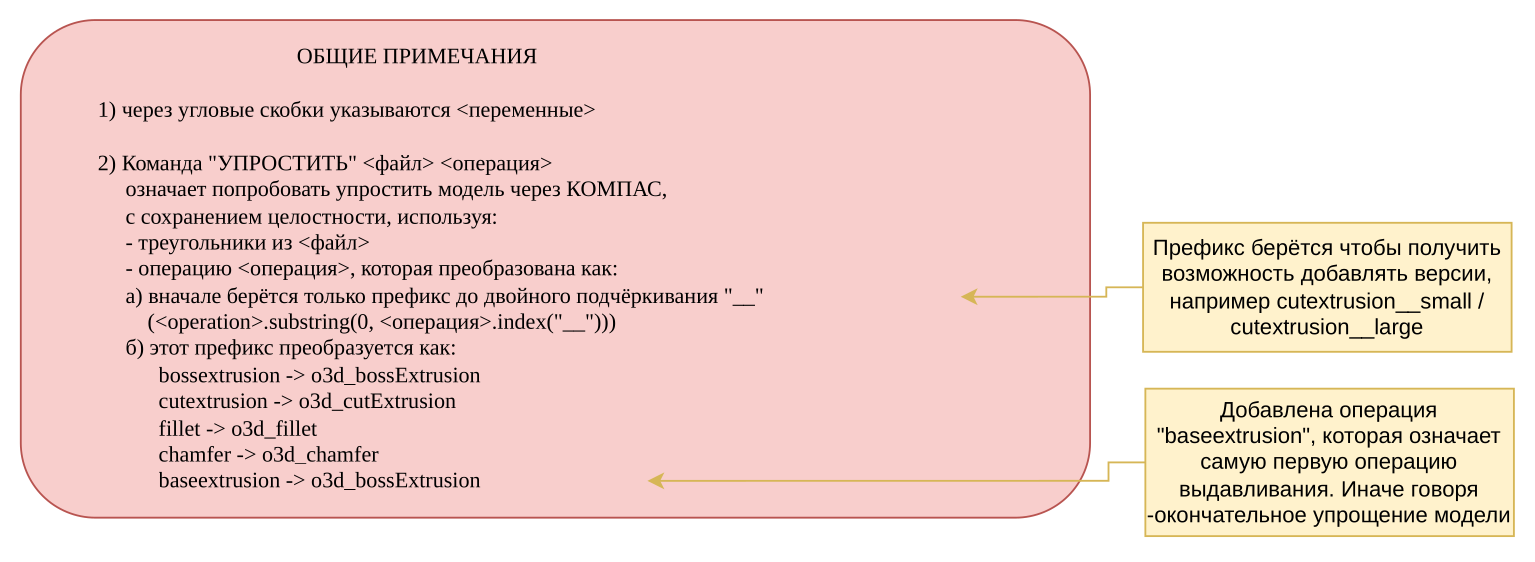
\includegraphics[width=0.5\linewidth]{figures/scheme_general.png}
    \caption{Схема работы main.exe - общее описание}
    \label{fig:placeholder}
\end{figure}

В полуавтоматическом режиме, программе в качестве параметров необходимо указать тип задачи (классификация / сегментация), тип операции, а также опциональные параметры постобработки. В ходе работы происходит препроцессинг исходного файла, вызывается нейронная сеть для выбранных типа задачи и операции, и результат сохраняется в виде файла в указанной папке. Вид файла зависит от типа задачи: в результате классификации получается файл meta.json, в котором указывается поле probability - уверенность нейронной сети в наличии выбранной операции в данной модели; в результате сегментации получается файл test\_0.stl, который содержит геометрию, которая, по мнению нейронной сети, относится к данному типу операции.

\begin{figure}
    \centering
    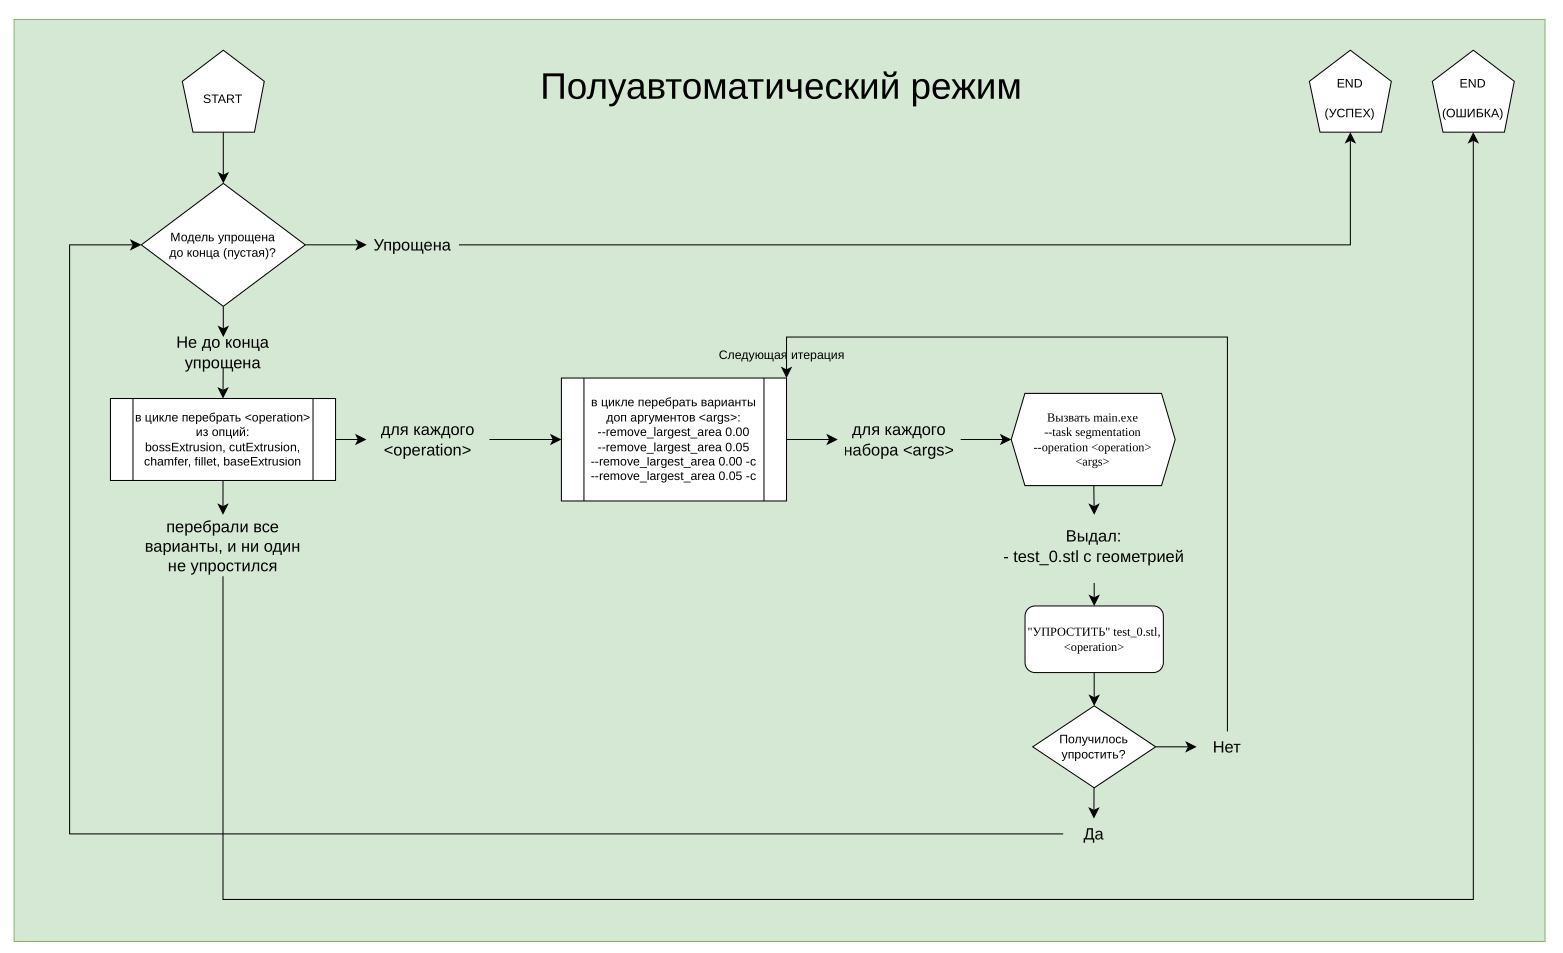
\includegraphics[width=0.5\linewidth]{figures/scheme_mode_semiauto.png}
    \caption{Схема работы main.exe - полуавтоматический режим}
    \label{fig:placeholder}
\end{figure}

В автоматическом режиме, программа получает исключенные из рассмотрения операции, а также опциональные параметры постобработки. В ходе работы она перебирает все доступные ей на данный момент нейронные сети, вызывая вначале классификаторы для каждого типа операции. На основе полученных уровней уверенности в наличии типа операции в модели выбирается тип операции, для которого будет вызвана процедура сегментации. Результатом являются сразу два файла: meta.json, содержащий выбранную операцию и уровень уверенности нейронной сети в наличии этой операции, а также test\_0.stl, который содержит геометрию, которая, по мнению нейронной сети, относится к данному типу операции.

\begin{figure}
    \centering
    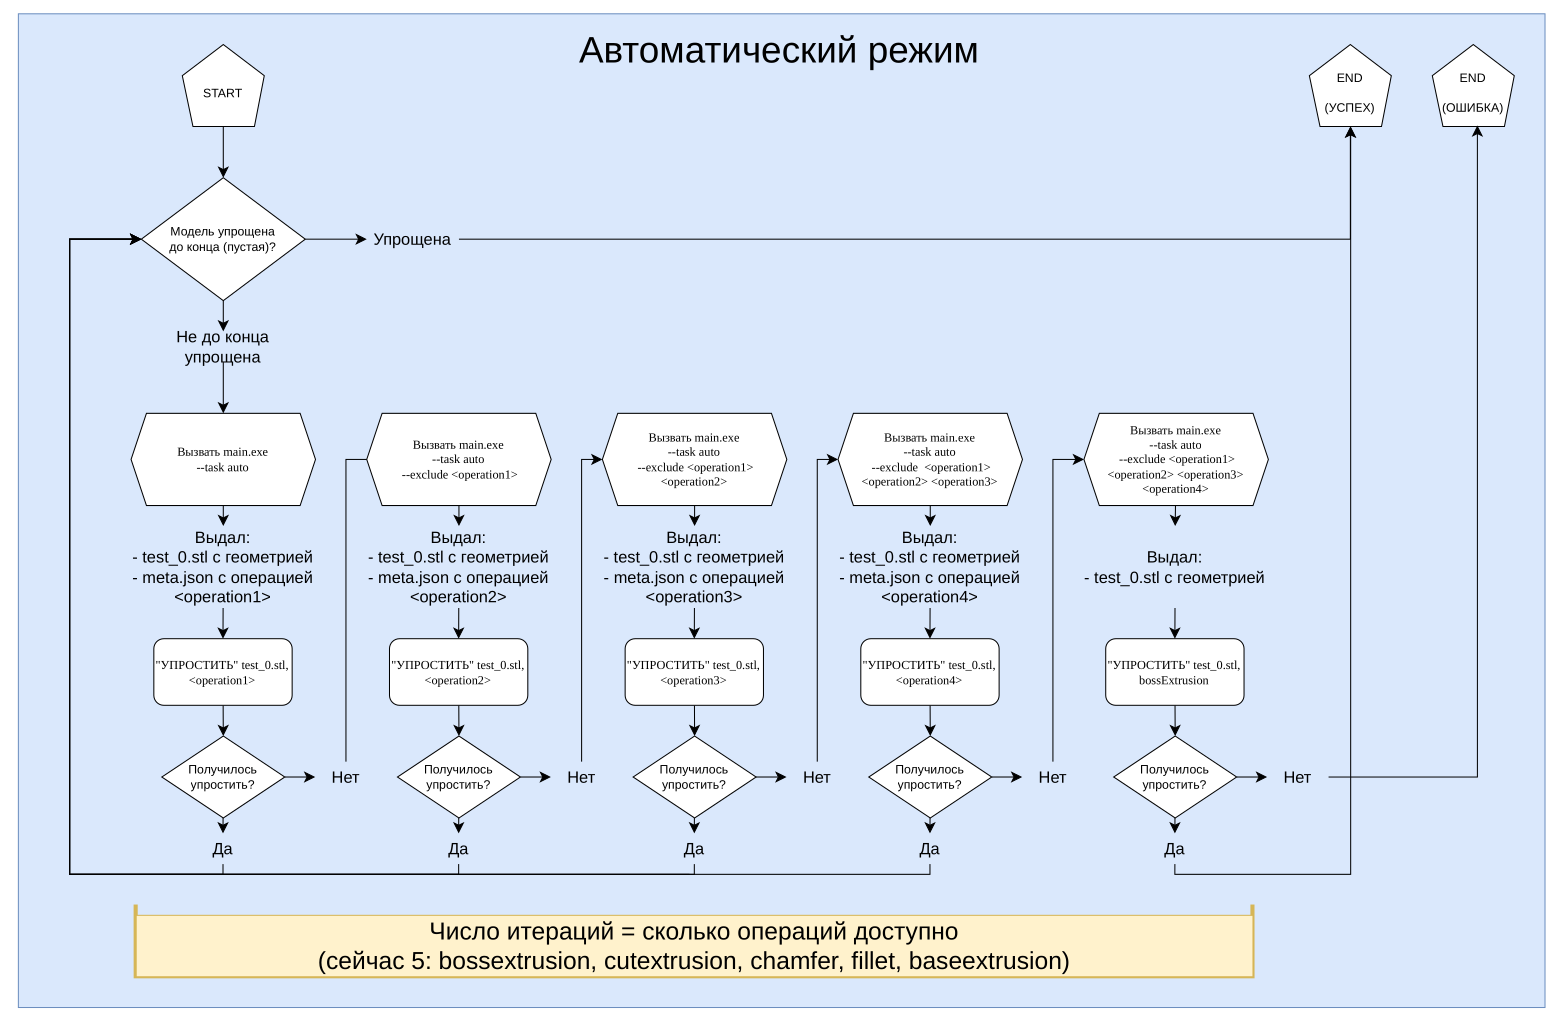
\includegraphics[width=0.5\linewidth]{figures/scheme_mode_auto.png}
    \caption{Схема работы main.exe - автоматический режим}
    \label{fig:placeholder}
\end{figure}

Таким образом, текущий рабочий подход может быть кратко сформулирован как гибридная сегментационно-классификационная схема с детерминированной CAD-постобработкой, мультипредставлением данных и явной интеграцией результатов в прикладной контур КОМПАС-3D.


\section{Экспериментальная проверка и анализ результатов}

TODO2

\subsection{Результаты обучения классификаторов и сегментаторов}

Ряд экспериментов подтвердил, что задача является решаемой. В частности, показатели обучения имеют стабильное, типовое поведение для подобных задач:

\begin{figure}
    \centering
    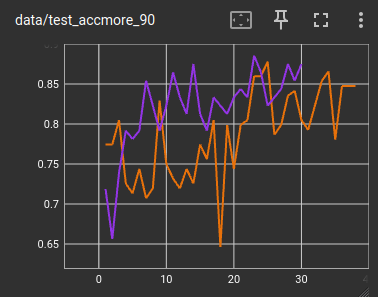
\includegraphics[width=0.5\linewidth]{figures/plot_cls_acc_1.png}
    \caption{График зависимости точности работы классификатора на тестовой выборке обучения от эпохи (bossExtrusion-оранжевый, fillet-фиолетовый)}
    \label{fig:placeholder}
\end{figure}

\begin{figure}
    \centering
    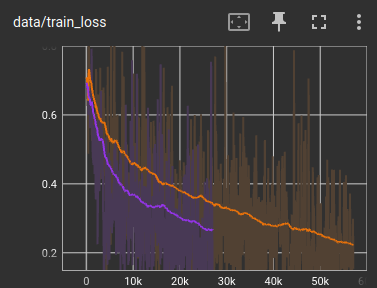
\includegraphics[width=0.5\linewidth]{figures/plot_cls_loss_1.png}
    \caption{График зависимости ошибки классификатора на обучающем датасете от эпохи обучения (bossExtrusion-оранжевый, fillet-фиолетовый)}
    \label{fig:placeholder}
\end{figure}

график accmore\_90 (Рисунок 4а) - показывает точность предсказания нейронной сети на тестовой выборке, чем больше значение - чем точнее предсказания; в случае успешного обучения, должен быть виден тренд на увеличение, что и происходит на картинке.
график train\_loss (Рисунок 4б) - показывает функцию ошибки на обучающем датасете, чем меньше значение - тем лучше обучена нейросеть; в случае успешного обучения, данный график должен стремиться к 0, что и происходит на картинке;
Таким образом, получено базовое подтверждение возможности использования STEP и текстового формата JSON для обучения нейросетей, так как обнаружен статистически извлекаемый сигнал: геометрия и последовательности операций содержат информацию, пригодную для машинного обучения и распознавания информации о типе операции.


После обучения в течение 50 эпох на датасете, полученном после очищения 21 464 моделей, получены следующие значения метрик:

\begin{table}[h]
\centering
\caption{Результаты сегментации}
\label{tab:segmentation-results}
\begin{tabular}{|l|c|c|c|}
\hline
\textbf{Операция} & \textbf{Доля верно определённых классов} & \textbf{Доля моделей, определённых на $\geq$90\%} & \textbf{Исходное распределение классов} \\
\hline
bossExtrusion & 78.4\% & 46.8\% & 59\% / 41\% \\
\hline
cutExtrusion (curve) & 96.8\% & 91.3\% & 56\% / 44\% \\
\hline
fillet & 93.6\% & 78.7\% & 40\% / 60\% \\
\hline
chamfer & 68.1\% & 53.125\% & 53\% / 47\% \\
\hline
\end{tabular}
\end{table}

“доля верно определённых классов” - число, равное отношению количества верно предсказанных классов рёбер к общему числу рёбер во всех моделях (сегментация), или отношению верно определённых наличия операции в модели с уверенностью выше 50\% к общему числу моделей (классификация);
“доля моделей, определённых на >=90\%” - число, равное количеству моделей, в которых 90\% всех рёбер были верно проклассифицированы;
“исходное распределение классов” - отношение количества классов в датасете (первое число - сколько рёбер / моделей соответствуют текущей операции, второе - сколько не соответствуют).
Все операции показали статистически значимое улучшение над тривиальной стратегией постоянного угадывания доминирующего класса. Это означает, что сеть научилась распознавать не только наиболее массовую операцию, но и часть остальных операций. Следует подчеркнуть, что данный результат нельзя без дополнительных проверок интерпретировать как достаточный уровень качества, в частности ввиду использования различных датасетов под каждую операцию в связи с её спецификой. Это содержательный baseline. Он показывает, что выбранная постановка для классификации операций дает сигнал выше случайного и выше простого частотного базиса. На данной стадии проекта это позволяет обоснованно переходить к улучшению и расширению датасетов и моделей.



\subsection{Анализ типовых ошибок и способов их устранения}

Этап 3 дал более содержательное качественное знание: было показано, что архитектуры на основе point cloud и DGCNN/LSTM-подобных блоков способны генерировать структурированное представление операции, но регрессионная часть остается ограничивающим фактором. В инженерной интерпретации это означает, что сеть понимает «что произошло», но недостаточно надежно восстанавливает «точно как именно это было задано численно». Такой результат дал проекту главное основание для корректной смены постановки.

Для сегментационного подхода наиболее конкретной зафиксированной метрикой является предварительная точность 84,5\% на тестовой выборке по операции fillet. Необходимо подчеркнуть несколько обстоятельств. Во-первых, это результат специализированного эксперимента, а не итоговая интегральная точность всей системы по всем операциям. Во-вторых, обучение проводилось на 1 726 моделях после дополнительных ограничений по сложности геометрии. В-третьих, метрика отражает точность предсказания типов ребер или элементов в задаче локальной сегментации, а не полноту восстановления дерева построения. Тем не менее именно этот результат является наиболее сильным количественным подтверждением правильности нового направления.

По результатам этапа также были определены косвенные признаки адекватности обучения: рост точности на тестовой выборке и убывание функции потерь на обучающей выборке без явных признаков немедленного переобучения. Для исследовательского этапа это важно, поскольку показывает, что модель продолжает извлекать информацию из данных и не исчерпала полезную емкость текущей выборки. Также был сделан вывод о необходимости более длительного обучения, а также о целесообразности дальнейшего расширения обучающего массива.

В то же время ряд примеров демонстрирует типичные ошибки. На одной из визуализаций отверстия ошибочно определяются как скругления; на другой видны отдельные ложноположительные ребра. Эти ошибки содержательно понятны. Геометрические признаки отверстий и скруглений частично пересекаются, особенно если рассматривать только локальные участки сетки без широкого контекста; небольшое количество ложноположительных ребер может быть следствием как ограниченного датасета, так и несовершенства автоматической разметки. Именно поэтому в отчете этапа 3 были предложены дальнейшие меры: ручная ревизия датасета, более однородное дробление моделей и возможный переход к альтернативным архитектурам вроде PointCNN.

В более общем смысле результаты 3 этапа следует трактовать как доказательство технологической реализуемости подхода, но не как завершенное решение задачи восстановления дерева построения. Проект уже прошел порог демонстрационной состоятельности: имеются данные, модели, исполняемый модуль, количественный результат по частной операции и четко выявленные ограничения. Следующий порог требует уже не только роста метрик, но и развития всего системного контура: качества данных, специализированных моделей, CAD-валидации и эксплуатационной надежности.



\subsection{Тестирование модуля main.exe на реальных деталях}

TODO0

\begin{figure}
    \centering
    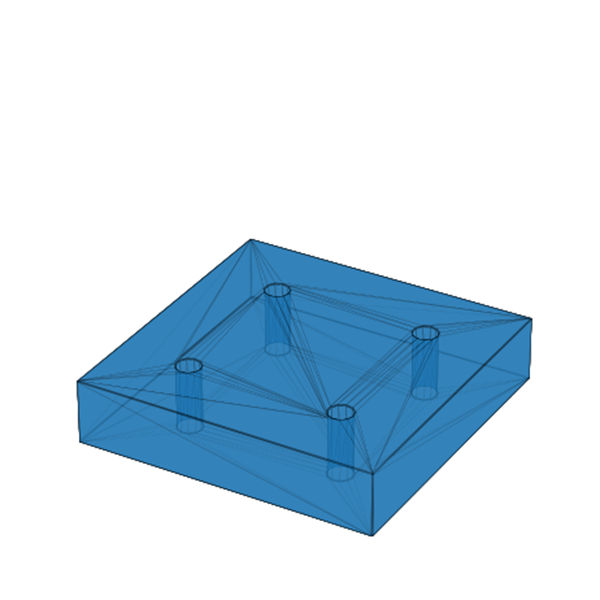
\includegraphics[width=0.5\linewidth]{figures/image.png}
    \caption{Enter Caption}
    \label{fig:placeholder}
\end{figure}

Шаги:

o3d\_bossExtrusion,
o3d\_cutExtrusion,
o3d\_fillet,
o3d\_fillet

cutExtrusion (отверстия):

\begin{figure}
    \centering
    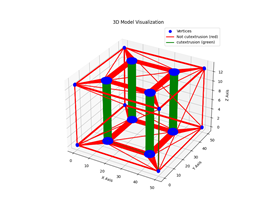
\includegraphics[width=0.5\linewidth]{figures/image2.png}
    \caption{Enter Caption}
    \label{fig:placeholder}
\end{figure}

\begin{figure}
    \centering
    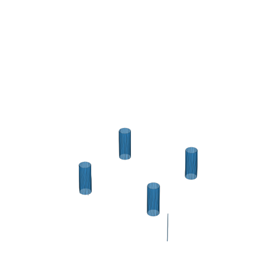
\includegraphics[width=0.5\linewidth]{figures/image3.png}
    \caption{Enter Caption}
    \label{fig:placeholder}
\end{figure}

\section{Оценка эффективности предложенного подхода}

Разработанный гибридный подход позволяет решить задачу восстановления истории построения с приемлемой точностью для основных операций. Полученные результаты (таблица~\ref{tab:seg-results}) демонстрируют, что:
\begin{itemize}
    \item для операций \texttt{fillet} и \texttt{cutExtrusion} точность сегментации превышает 90\%;
    \item классификатор для \texttt{fillet} достигает 90.6\% accuracy;
    \item даже для менее представленной операции \texttt{chamfer} точность выше случайного угадывания.
\end{itemize}

Преимущества предложенного решения:
\begin{itemize}
    \item Модульность: можно обучать и добавлять новые операции независимо.
    \item Интерпретируемость: сегментация позволяет визуально контролировать результат.
    \item Интеграция с CAD-ядром: точные параметры вычисляются детерминированно, что повышает надёжность.
\end{itemize}

Ограничения:
\begin{itemize}
    \item Зависимость от качества датасета (дисбаланс, сложность моделей).
    \item STL теряет инженерную семантику, что ограничивает точность параметрической реконструкции.
    \item В текущей версии поддерживаются только четыре типа операций.
\end{itemize}

Тем не менее, полученные результаты подтверждают принципиальную осуществимость подхода и его пригодность для дальнейшего масштабирования.



\section{Обсуждение ограничений и путей дальнейшего развития}

TODO2

На данный момент можно четко выделить два класса проблем, оказывающих влияние на точность, воспроизводимость и скорость развития системы.

Проблема качества и состава датасета. Датасет содержит неполные и неоднородные примеры, сильный дисбаланс по классам, чрезмерно сложные исходные модели. Имеющегося набора данных недостаточно, так как состав датасета по операциям неравномерен, часть примеров невалидна или непригодна для обучения, а истории построения часто используют не-атомарные операции, потому непригодные для обучения нейронной сети, которая должна делать отдельные простые шаги, собирая всё в итоге в дерево построения. Для некоторых операций из большого корпуса моделей удавалось использовать лишь небольшую долю наблюдений из-за отсутствия нужных шагов, пустых STL либо чрезмерной сложности исходных объектов. Решение состоит в жесткой валидации наборов, фильтрации нерепрезентативных примеров, выделении специализированных поддатасетов по операциям и формировании отдельного корпуса простых моделей для сегментации и параметризации. 

Проблема ограниченности STL как источника инженерной семантики. STL описывает поверхность как триангуляцию, но не содержит явной CAD-семантики граней, эскизов и ограничений. Решение — постепенный переход к комбинированному использованию STL для распознавания и STEP/B-Rep для уточнения инженерного смысла.


\begin{enumerate}
    \item Во время триангуляции, треугольники могут быть ориентированы по часовой или против часовой стрелки. На данный момент, ориентация определяется каким-то внутренним алгоритмом и, по сути, случайна. Можно использовать данный аспект как способ передать метаинформацию в модель - например, ориентировать треугольники по-разному в зависимости от типа порождающей поверхности, или ориентировать иначе треугольники на границе (стыке) двух поверхностей для облегчения детекции границ.
    \item Сейчас на инференсе STEP используется только для того, чтобы обеспечить известный алгоритм триангуляции, с фиксированным числом треугольников и рёбер. Если выбрать правильный метод конвертации (с равномерным заполнением точек), то можно любой входной файл конвертировать вначале в Point cloud, а потом в STL: STP -> Point cloud -> STL, STL -> Point cloud -> STL, …, обеспечив поддержку произвольного 3D формата. Таким образом, целесообразно добавить поддержку STL и/или Point cloud на инференсе путём преобразования всех данных (как на этапе обучения, так и на этапе инференса) - например, в Point cloud.
    \item Сейчас для обучения используется только последний шаг модели - берется геометрия, полученная на последнем шаге, и только она раскрашивается и используется при обучении. Так как триангуляция сильно меняется практически при любой операции, можно увеличить датасет используя, например, каждый второй шаг, или вообще каждый шаг построения модели как отдельную модель. Таким же образом можно будет использовать модели, у которых последний шаг слишком сложен, чтобы входить в обучающую выборку (слишком много треугольников) - использовать модель с первых N шагов, в которой треугольников становиться уже достаточно мало.
    \item Сейчас обучение происходит так, что предсказываются сразу все грани, порожденные выбранной операцией. Можно попробовать применить другой способ обучения, при котором обучение происходит только на последних последовательных однотипных операциях. Для примера возьмём cutExtrusion. Вместо того, чтобы искать сразу все вырезания, можно попробовать искать только все последние последовательные вырезания. Так, если будет 4 операции: bossExtrusion, cutExtrusion, bossExtrusion (который сделан поверх первого вырезания и сломавший его форму), а потом cutExtrusion - то мы не будем вводить штрафы для нейронной сети за то, что она не признала первое отверстие, которые было “сломано” выдавливанием, как мы бы делали в наивном подходе. Также, мы попутно решаем проблему “стола” - это если к столешнице были приделаны 4 ножки - то мы будем позволять bossExtrusion находить все 4 ножки сразу, независимо от того, в каком порядке их решил сделать исходный разработчик.
    \item Нейросеть фундаментально работает с рёбрами, и поэтому необходим алгоритм, преобразующий окрашенные рёбра в окрашенные треугольники. Сейчас в итоговый test\_0.stl попадают только те треугольники, которые содержат хотя бы 2 покрашенных ребра. Возможно, будет лучше выбирать только те, где покрашены все 3 ребра - хотя даже в таком случае (например, в случае тетраэдра) невозможно выбрать все грани кроме ровно одной. Возможно, стоит разбивать такие грани на более мелкие треугольники, и позволять нейросети таким образом выражать степень уверенности в каждой отдельной грани.
    \item ожно добавить в постобработке опцию для фильтрации треугольников не только по их площади (как происходит сейчас), а ещё, например, по длине, по углу наклона, по расстоянию от центра модели и прочим 3D характеристикам, которые получится найти - это позволит исключить ситуации, в которых нейронная сеть случайно выдала какой-то один длинный или дальний треугольник (например, находящийся сильно дальше от скучкованных всех других).
    \item Для всех операций можно обучить 3 версии нейросетей: одну для операции по изогнутым контурам, вторую для операции по контурам из отрезков, и третью для смешанных операций. Сейчас, так как число треугольников для этих трёх случаев сильно отличается, то нейронная сеть, обучающаяся на всех трёх случаях разом, стремится приоритизировать именно скруглённые контуры.
    \item В дальнейшем требуется дообучить остальные основные операции, такие как: rotated, linear\_pattern, axis3D, mirror\_pattern и пр.
    \item Можно применить скомбинированный принцип обучения: при наличии двух датасетов, один из которых большой, но “грязный”, а второй относительно маленький, но собранный и проверенный вручную, возможно обучить нейросеть вначале только на большом, чтобы она выучила основные паттерны и структуру, а потом уже дообучить на хорошем, чтобы она смогла разобраться в деталях и нюансах.
    \item Можно создать скрипт для автоматической оценки качества нейронной сети: ввести и зафиксировать конкретные метрики, такие как “процент разбирающихся в ноль моделей”, или “суммарное число шагов, на которое получилось упростить набор моделей”, или “общий объём удалённой части тела”, и запускать периодически его в связке с КОМПАС-3D для валидации и оценки новых вариантов и версий main.exe.
    \item Можно сделать отдельный программный модуль, который будет обучать и использовать нейронную сеть, которая при получении глобального набора треугольников "операции" будет выдавать границы между ними. Таким образом, мы сможем, получив вывод текущего сегментатора (например, что вся модель была сделана исключительно из bossExtrusion) вызвать этот “разделитель” и найти конкретно треугольники, относящиеся к каждому отдельному шагу.
    \item Наконец, можно увеличить количество треугольников в моделях, или размер самих нейронных сетей (с учетом увеличения вычислительных затрат), а также подобрать гиперпараметры обучения для улучшения качества моделей.
\end{enumerate}




\backmatter
% META: DONE.1

\chapternoindex{Заключение}

В рамках данной выпускной квалификационной работы достигнута поставленная цель: разработан программный модуль «НейроКОМПАС-3D», интегрируемый со средой КОМПАС-3D и работающий локально на стороне клиента. Модуль по анализу геометрии модели позволяет реконструировать последовательность породивших её формообразующих операций с использованием методов машинного обучения.

В ходе выполнения работы решены все сформулированные задачи. Основные научные и практические результаты:

\begin{enumerate}
    \item Проведён всесторонний анализ предметной области, выявлены ключевые ограничения существующих подходов (неоднозначность интерпретации, чувствительность к шумам, отсутствие обучаемости). Обоснована необходимость гибридной архитектуры.
    
    \item Сформирован и очищен репрезентативный датасет из 10483 моделей (исходно 22275), каждая из которых содержит полную историю построения в формате JSON и геометрические представления (STEP/STL). Разработан конвейер автоматической разметки рёбер для обучения сегментационных нейросетей.
    
    \item Обоснован и реализован гибридный подход, сочетающий нейросетевую сегментацию (MeshCNN) для локализации следов операций с детерминированным вычислением параметров в CAD-ядре. Подход снимает с нейросети задачу точной регрессии параметров, чувствительной к масштабу и системе координат.
    
    \item Разработаны и обучены нейросетевые классификаторы и сегментаторы для четырёх базовых операций: \texttt{bossExtrusion} (выдавливание), \texttt{cutExtrusion} (вырезание), \texttt{fillet} (скругление), \texttt{chamfer} (фаска). На тестовых выборках достигнута точность классификации до 88.2\% (для \texttt{chamfer}) и точность сегментации (IoU) до 0,84 (для \texttt{chamfer}), доля моделей с точностью сегментации не менее 90\% составила 88,3\% для фаски и 83,7\% для скругления.
    
    \item Создан исполняемый модуль, реализующий полный цикл инференса: адаптивную триангуляцию STEP-файла, нормализацию сетки до фиксированного числа рёбер (2250), вызов обученных классификаторов/сегментаторов в автоматическом или ручном режиме, постобработку (фильтрация по площади, выделение связного компонента) и подготовку результатов (STL выделенной геометрии, JSON с типом операции и уверенностью). Модуль интегрирован с КОМПАС-3D через API и позволяет итеративно упрощать модель путём удаления распознанных операций.
\end{enumerate}

Разработанный прототип перешёл в стадию опытной эксплуатации в рамках договора с ООО «АСКОН-Системы проектирования» и показал работоспособность на наборе реальных деталей (примеры приведены в приложении Г). Модуль применим для упрощения базовых 3D-моделей, восстановления параметрической истории импортированных моделей, а также для обучения инженеров-конструкторов.

\textbf{Перспективы дальнейшего развития:}
\begin{itemize}
    \item увеличение датасета за счёт использования всех промежуточных шагов построения (потенциальное увеличение в 5-10 раз);
    \item поддержка новых типов операций (вращение, линейные и круговые массивы, кинематические операции);
    \item улучшение постобработки (фильтрация по длине рёбер, по расстоянию от центра масс);
    \item раздельное обучение для прямолинейных и криволинейных контуров с целью устранения дисбаланса плотности триангуляции;
    \item автоматическая оценка качества через API КОМПАС-3D (процент успешно упрощённых моделей, среднее количество восстановленных шагов);
    \item увеличение разрешения сетки (до 4500-6000 рёбер) и ёмкости нейросетевой архитектуры для распознавания мелких деталей.
\end{itemize}

Таким образом, представленная работа вносит вклад в решение актуальной задачи восстановления истории построения параметрических моделей и демонстрирует эффективность гибридного подхода, сочетающего машинное обучение с детерминированными алгоритмами CAD-систем. Полученные результаты могут служить основой для дальнейших исследований и промышленного внедрения.


\chapternoindex{Приложение A}

TODO1

\chapternoindex{Приложение B}

TODO1

\chapternoindex{Приложение C}

TODO1

\printbib

\end{document}